\section{Functional Requirements}

\subsection{System Functional Overview}

\subsubsection{Screen Flow}

Do hệ thống phục vụ nhiều nhóm người dùng với luồng thao tác khác nhau,
luồng màn hình được tách thành 7 sơ đồ riêng theo từng nhóm actor để đảm
bảo dễ đọc.

\begin{figure}[htbp]
    \centering
    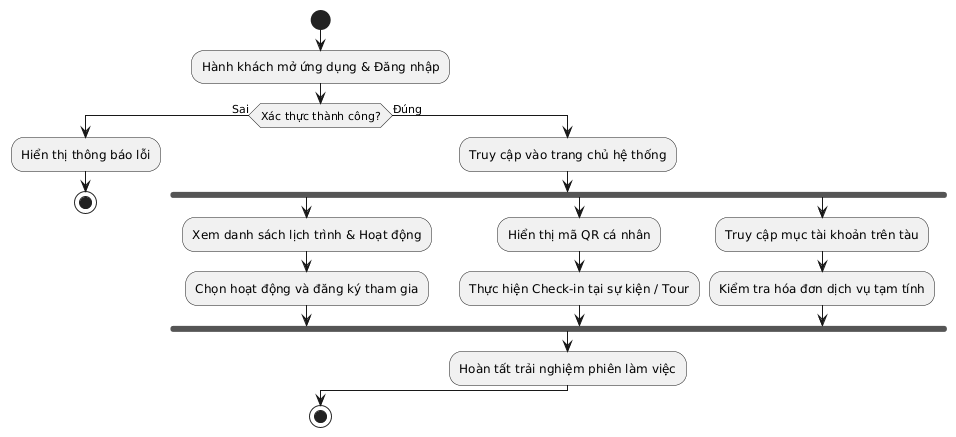
\includegraphics[width=0.9\textwidth]{chapters/ch3/screenflow-passenger.png}
    \caption{Luồng màn hình — Hành khách}
    \label{fig:screenflow-passenger}
\end{figure}

\begin{figure}[htbp]
    \centering
    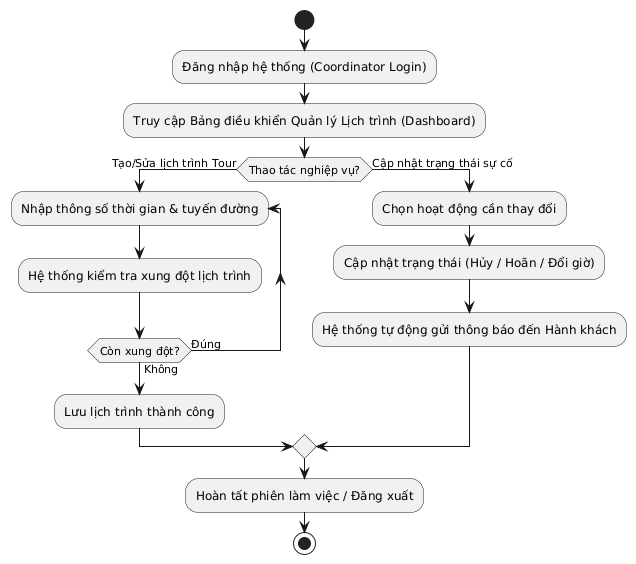
\includegraphics[width=0.9\textwidth]{chapters/ch3/screen-flow-coordinator.png}
    \caption{Luồng màn hình — Điều phối lịch trình}
    \label{fig:screenflow-coordinator}
\end{figure}

\begin{figure}[htbp]
    \centering
    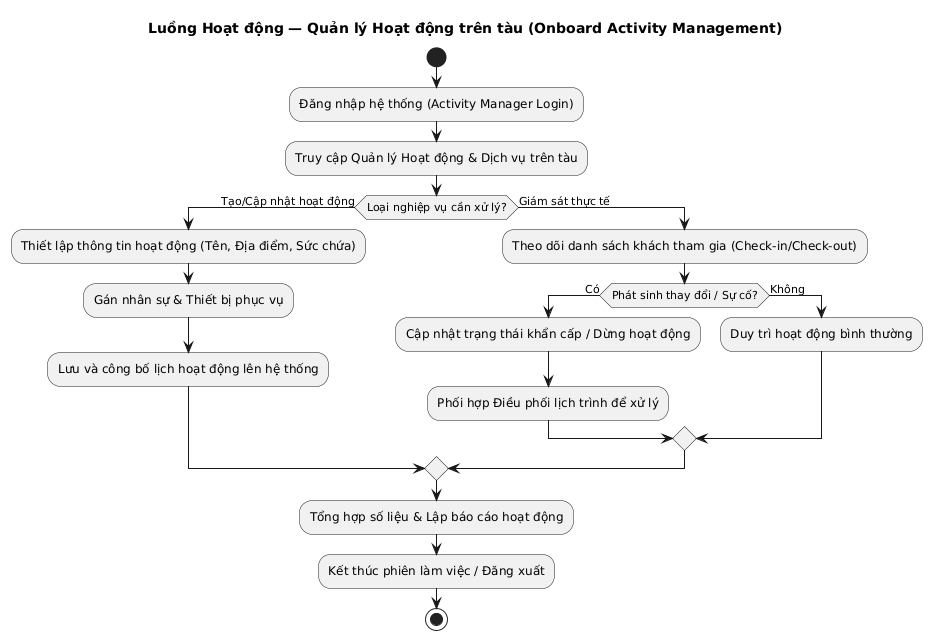
\includegraphics[width=0.9\textwidth]{chapters/ch3/screen-flow-activity.png}
    \caption{Luồng màn hình — Quản lý hoạt động trên tàu}
    \label{fig:screenflow-activity}
\end{figure}

\begin{figure}[htbp]
    \centering
    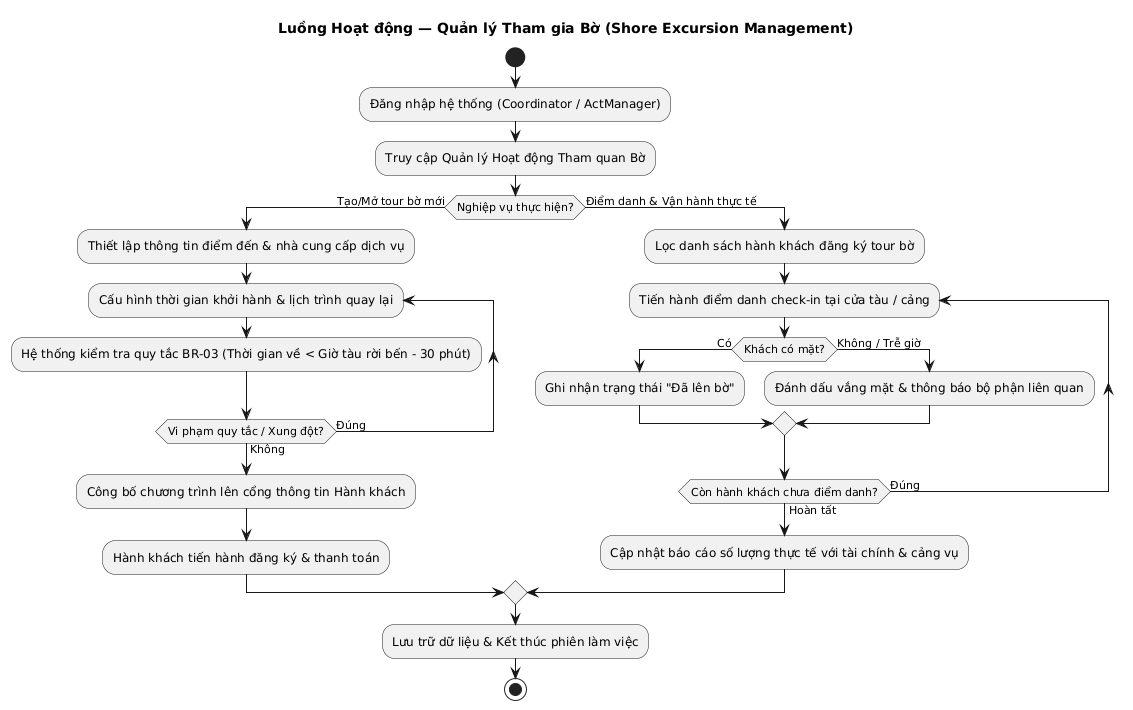
\includegraphics[width=0.9\textwidth]{chapters/ch3/screen-flow-excursion.png}
    \caption{Luồng màn hình — Quản lý tham quan bờ}
    \label{fig:screenflow-excursion}
\end{figure}

\begin{figure}[htbp]
    \centering
    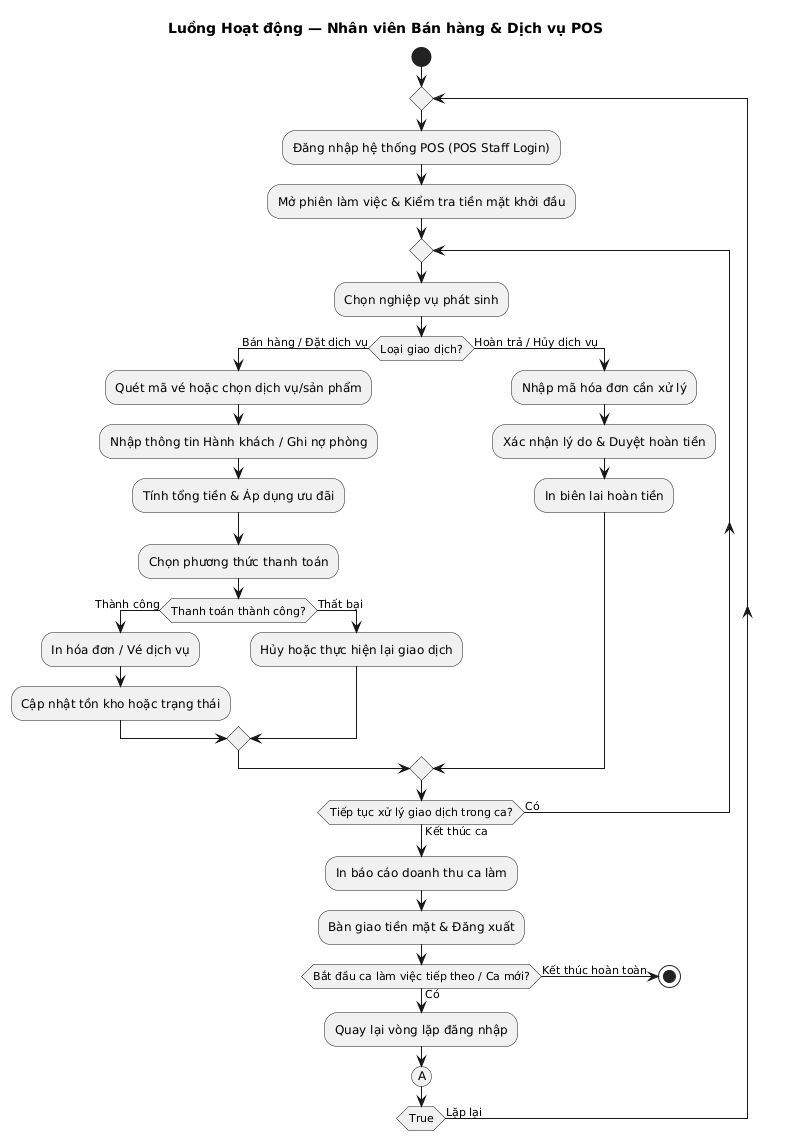
\includegraphics[width=0.9\textwidth]{chapters/ch3/screen-flow-pos.png}
    \caption{Luồng màn hình — Nhân viên bán hàng \& dịch vụ (POS)}
    \label{fig:screenflow-pos}
\end{figure}

\begin{figure}[htbp]
    \centering
    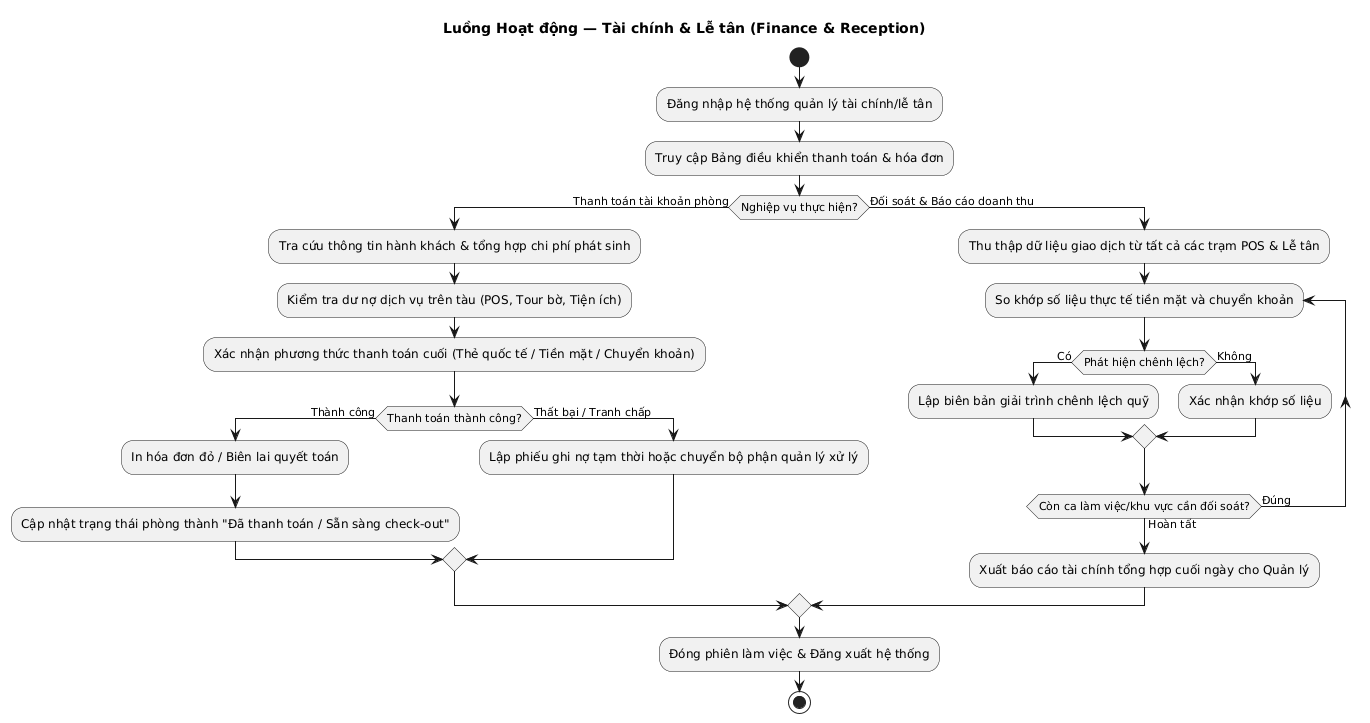
\includegraphics[width=0.9\textwidth]{chapters/ch3/screen-flow-finance.png}
    \caption{Luồng màn hình — Tài chính \& Lễ tân}
    \label{fig:screenflow-finance}
\end{figure}

\begin{figure}[htbp]
    \centering
    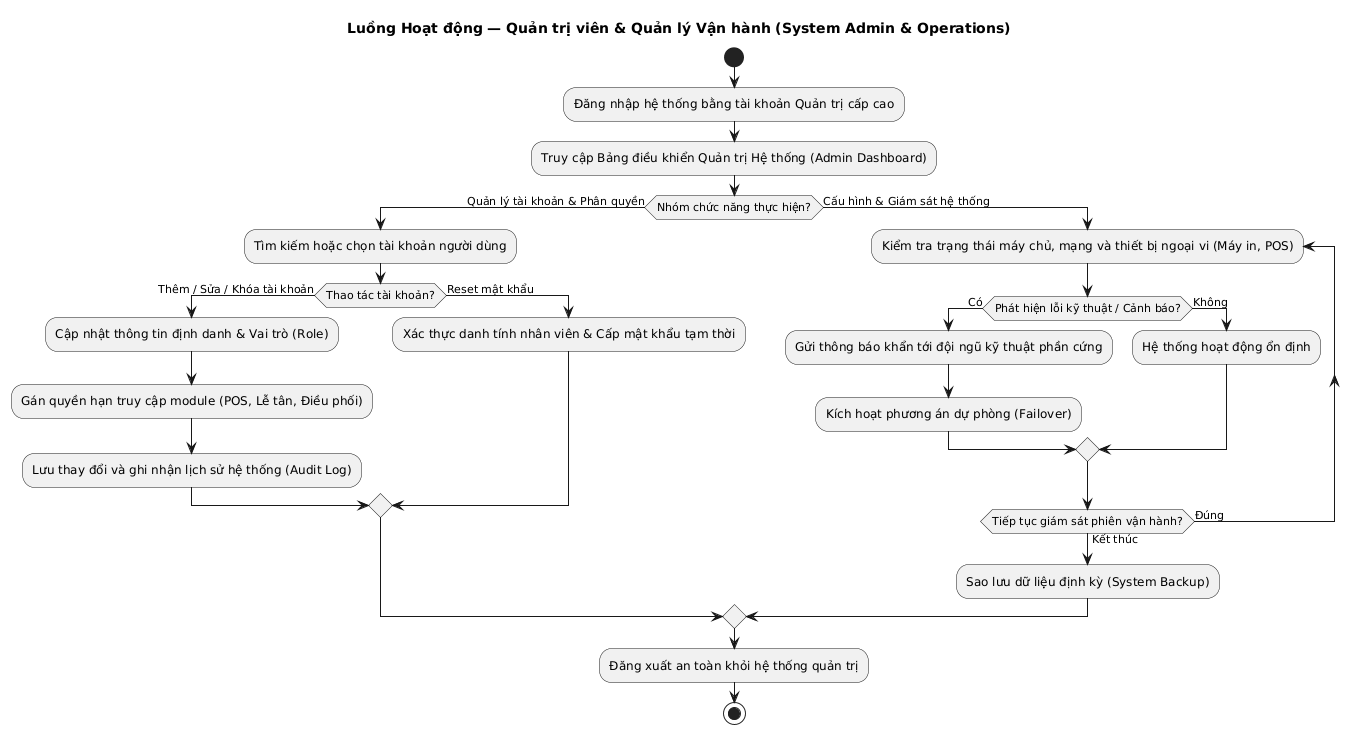
\includegraphics[width=0.9\textwidth]{chapters/ch3/screen-flow-operations-admin.png}
    \caption{Luồng màn hình — Quản lý vận hành \& Quản trị viên hệ thống}
    \label{fig:screenflow-operations-admin}
\end{figure}

\FloatBarrier
\subsubsection{Screen Descriptions}

\begin{longtable}{|p{0.6cm}|p{3.2cm}|p{3.2cm}|p{6.5cm}|}
    \hline
    \textbf{\#} & \textbf{Feature} & \textbf{Screen} & \textbf{Mô tả} \\
    \hline
    \endfirsthead
    \hline
    \textbf{\#} & \textbf{Feature} & \textbf{Screen} & \textbf{Mô tả} \\
    \hline
    \endhead
    1 & Xác thực & Login & Cho phép tất cả actor đăng nhập theo vai trò \\
    \hline
    2 & Lịch trình & Trang lịch trình & Hành khách xem lịch trình theo
    ngày, cảng ghé thăm \\
    \hline
    3 & Hoạt động & Danh sách hoạt động & Hiển thị hoạt động trên tàu và
    tham quan bờ, lọc miễn phí/trả phí \\
    \hline
    4 & Chi tiết hoạt động & Chi tiết hoạt động & Thông tin chi tiết: thời
    gian, địa điểm, sức chứa, phí \\
    \hline
    5 & Đăng ký & Form đăng ký & Hành khách đăng ký tham gia hoạt
    động/tham quan \\
    \hline
    6 & Check-in & Màn hình check-in & Quét QR/thẻ/RFID-NFC để xác nhận
    tham gia \\
    \hline
    7 & Chi phí & Hóa đơn tạm tính & Hành khách xem các khoản chi phí đã
    phát sinh \\
    \hline
    8 & Thông báo & Notification & Danh sách thông báo về lịch trình, hoạt
    động \\
    \hline
    9 & Phản hồi & Form phản hồi & Gửi đánh giá sau hoạt động / cuối
    chuyến \\
    \hline
    10 & Quản lý tour & Manage Tour & Điều phối tạo/sửa chuyến du lịch
    nhiều ngày \\
    \hline
    11 & Quản lý lịch trình & Manage Itinerary & Thiết lập lịch trình chi
    tiết theo từng ngày \\
    \hline
    12 & Quản lý cảng & Manage Port & Thiết lập giờ cập bến/rời bến từng
    cảng \\
    \hline
    13 & Tạo hoạt động & Create Activity & Quản lý hoạt động tạo mới hoạt
    động trên tàu \\
    \hline
    14 & Tạo tham quan bờ & Create Excursion & Quản lý tham quan bờ tạo
    mới chuyến tham quan \\
    \hline
    15 & Danh sách đăng ký & Registration List & Xem/giám sát danh sách
    hành khách đã đăng ký \\
    \hline
    16 & Bán hàng POS & POS Screen & Nhân viên ghi nhận giao dịch dịch
    vụ/sản phẩm \\
    \hline
    17 & Xác thực POS & Authentication Scan & Quét QR/thẻ/RFID-NFC để xác
    thực hành khách tại POS \\
    \hline
    18 & Quản lý tài khoản trên tàu & Onboard Account & Tài chính xem/quản
    lý số dư theo hành khách/phòng \\
    \hline
    19 & Đối soát & Reconciliation & Đối soát giao dịch POS, xử lý tranh
    chấp \\
    \hline
    20 & Hóa đơn cuối chuyến & Final Invoice & Xuất hóa đơn tổng hợp cuối
    chuyến đi \\
    \hline
    21 & Dashboard vận hành & Operations Dashboard & Biểu đồ hoạt động,
    doanh thu, sức chứa \\
    \hline
    22 & Quản lý user & Manage User & Admin CRUD tài khoản người dùng \\
    \hline
    23 & Cấu hình chính sách & Policy Config & Admin cấu hình chính sách
    đăng ký/hủy/hoàn tiền \\
    \hline
    24 & Quản lý thiết bị & Device Management & Admin quản lý thiết bị
    QR/RFID/NFC/BLE \\
    \hline
    \caption{Mô tả các màn hình chính}
    \label{tab:screen-descriptions}
\end{longtable}

\subsubsection{Screen Authorization}

\begin{longtable}{|p{3.3cm}|p{1cm}|p{1cm}|p{1.3cm}|p{1.3cm}|p{0.9cm}|p{1.1cm}|p{1.1cm}|p{0.9cm}|}
    \hline
    \textbf{Screen} & \textbf{HK} & \textbf{ĐP} & \textbf{QLHĐ} & \textbf{QLTQ}
    & \textbf{NVPOS} & \textbf{TC} & \textbf{VH} & \textbf{AD} \\
    \hline
    \endfirsthead
    \hline
    \textbf{Screen} & \textbf{HK} & \textbf{ĐP} & \textbf{QLHĐ} & \textbf{QLTQ}
    & \textbf{NVPOS} & \textbf{TC} & \textbf{VH} & \textbf{AD} \\
    \hline
    \endhead
    Login & x & x & x & x & x & x & x & x \\ \hline
    Trang lịch trình & x & x & & & & & x & \\ \hline
    Danh sách hoạt động & x & & x & x & & & x & \\ \hline
    Đăng ký hoạt động & x & & & & & & & \\ \hline
    Check-in & x & & x & x & x & & & \\ \hline
    Hóa đơn tạm tính & x & & & & & x & & \\ \hline
    Quản lý tour & & x & & & & & x & \\ \hline
    Quản lý cảng & & x & & & & & x & \\ \hline
    Tạo hoạt động & & & x & & & & & \\ \hline
    Tạo tham quan bờ & & & & x & & & & \\ \hline
    Bán hàng POS & & & & & x & & & \\ \hline
    Quản lý tài khoản trên tàu & & & & & & x & x & \\ \hline
    Đối soát & & & & & & x & x & \\ \hline
    Xuất hóa đơn & & & & & & x & & \\ \hline
    Dashboard vận hành & & & & & & & x & x \\ \hline
    Quản lý user & & & & & & & & x \\ \hline
    Cấu hình chính sách & & & & & & & & x \\ \hline
    Quản lý thiết bị & & & & & & & & x \\ \hline
    \caption{Phân quyền truy cập màn hình (HK: Hành khách, ĐP: Điều phối,
    QLHĐ: Quản lý hoạt động, QLTQ: Quản lý tham quan, NVPOS: Nhân viên
    POS, TC: Tài chính, VH: Vận hành, AD: Admin)}
    \label{tab:screen-authorization}
\end{longtable}

\subsubsection{Non-Screen Functions}

\begin{longtable}{|p{0.6cm}|p{4cm}|p{2.8cm}|p{6cm}|}
    \hline
    \textbf{\#} & \textbf{Feature} & \textbf{System Function} & \textbf{Mô tả} \\
    \hline
    \endfirsthead
    \hline
    \textbf{\#} & \textbf{Feature} & \textbf{System Function} & \textbf{Mô tả} \\
    \hline
    \endhead
    1 & Đồng bộ giao dịch ngoại tuyến & Background Job & Tự động đồng bộ
    giao dịch POS lưu tạm khi có kết nối mạng trở lại \\
    \hline
    2 & Thông báo tự động thay đổi lịch trình & Event Trigger & Tự động
    gửi thông báo khi lịch trình được điều phối cập nhật \\
    \hline
    3 & Kiểm tra sức chứa hoạt động & Validation Job & Kiểm tra và khóa
    đăng ký khi hoạt động đạt sức chứa tối đa \\
    \hline
    4 & Ước tính vị trí BLE & Background Job (tùy chọn) & Định kỳ cập nhật
    vị trí khu vực của hành khách qua thiết bị BLE \\
    \hline
    5 & Xuất báo cáo vận hành & API Endpoint & Cho phép quản lý vận hành
    xuất báo cáo dạng Excel/PDF sau chuyến đi \\
    \hline
    \caption{Các chức năng không có màn hình (chạy nền/hệ thống)}
    \label{tab:non-screen-functions}
\end{longtable}

\subsubsection{Entity Relationship Diagram}

\begin{figure}[H]
    \centering
    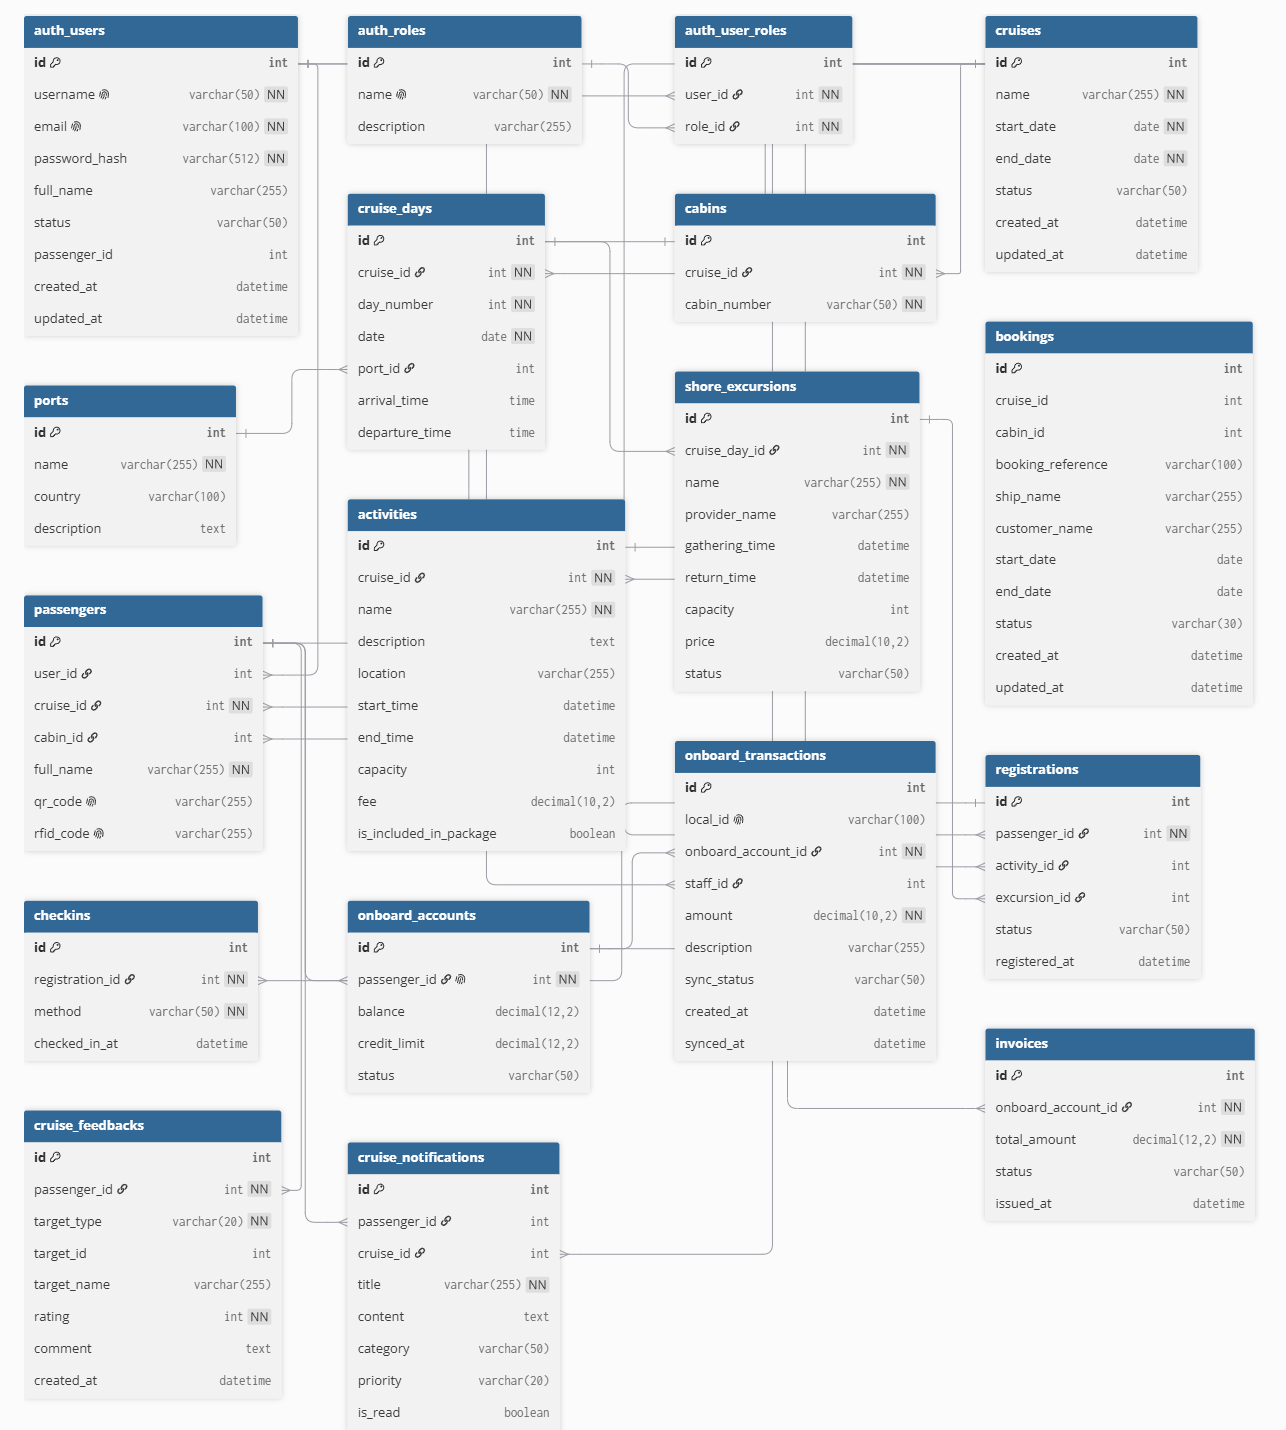
\includegraphics[width=0.95\textwidth]{images/ERD.png}
    \caption{Sơ đồ ERD mức khái niệm}
    \label{fig:erd-conceptual}
\end{figure}

\subsection{Xác thực (Authentication)}

\subsubsection{Đăng nhập}
\textbf{Actor:} Tất cả actor \\
\textbf{Function trigger:} Người dùng nhập thông tin đăng nhập (hoặc quét
thẻ/QR nếu là thiết bị POS/Tablet)

\textbf{Function description:}
\begin{itemize}
    \item Purpose: Xác thực người dùng và điều hướng theo vai trò.
    \item Data processing: Xác thực thông tin đăng nhập, tạo phiên làm
    việc (JWT token).
\end{itemize}

\textbf{Function Details:}
\begin{itemize}
    \item Nếu đăng nhập thành công → điều hướng tới Dashboard/Home theo
    role.
    \item Nếu thất bại → hiển thị thông báo lỗi.
    \item Business Rules: Áp dụng RBAC (Role-Based Access Control) — mỗi
    role chỉ thấy chức năng thuộc quyền của mình.
\end{itemize}

\begin{figure}[htbp]
    \centering
    \fbox{\parbox[c][3.0cm][c]{0.52\textwidth}{\centering \textbf{Mockup màn hình Login}\\ \small{(placeholder: mockup-login.png)}}}
    \caption{Mockup màn hình Login}
    \label{fig:mockup-login}
\end{figure}

\subsection{Quản lý Lịch trình (Itinerary Management)}

\subsubsection{Tạo chuyến du lịch nhiều ngày}
\textbf{Actor:} Điều phối lịch trình \\
\textbf{Function trigger:} Điều phối viên chọn "Tạo tour mới"

\textbf{Function description:}
\begin{itemize}
    \item Purpose: Thiết lập một chuyến du lịch mới với lịch trình nhiều
    ngày.
    \item Interface: Form nhập tên tour, ngày khởi hành, ngày kết thúc,
    danh sách cảng ghé thăm theo từng ngày.
    \item Data processing: Lưu thông tin tour và lịch trình vào database,
    tạo bản ghi Itinerary cho từng ngày.
\end{itemize}

\textbf{Function Details:}
\begin{itemize}
    \item Validation: Ngày kết thúc phải sau ngày bắt đầu; mỗi ngày chỉ có
    tối đa 1 cảng chính.
    \item Business Rules: Không được tạo 2 tour trùng thời gian trên cùng
    một tàu.
    \item Normal Case: Điều phối viên nhập đầy đủ thông tin → lưu thành
    công → hệ thống hiển thị thông báo.
    \item Abnormal Case: Thiếu trường bắt buộc → hiển thị lỗi validation.
\end{itemize}

% \begin{figure}[h]
%     \centering
%     \includegraphics[width=0.8\textwidth]{images/mockup-create-tour.png}
%     \caption{Mockup màn hình Tạo tour / lịch trình nhiều ngày}
% \end{figure}

\subsubsection{Quản lý cảng ghé thăm}
\textbf{Actor:} Điều phối lịch trình \\
\textbf{Function trigger:} Điều phối viên chọn một ngày trong lịch trình
→ "Thêm cảng"

\textbf{Function description:}
\begin{itemize}
    \item Purpose: Thiết lập thời gian tàu cập bến và rời bến tại từng
    cảng.
    \item Data processing: Lưu thông tin cảng, giờ cập bến, giờ rời bến
    vào bản ghi Itinerary tương ứng.
\end{itemize}

\textbf{Function Details:}
\begin{itemize}
    \item Validation: Giờ rời bến phải sau giờ cập bến.
    \item Business Rules: Giờ tập trung quay lại tàu phải được thiết lập
    trước giờ rời bến ít nhất 30 phút.
    \item Normal Case: Nhập thông tin cảng hợp lệ → lưu thành công.
    \item Abnormal Case: Giờ không hợp lệ → hiển thị lỗi.
\end{itemize}


\subsubsection{Cập nhật thay đổi lịch trình}
\textbf{Actor:} Điều phối lịch trình \\
\textbf{Function trigger:} Điều phối viên chỉnh sửa lịch trình đã tạo do
thời tiết/vận hành

\textbf{Function description:}
\begin{itemize}
    \item Purpose: Cập nhật thay đổi và thông báo đến các bên liên quan.
    \item Data processing: Cập nhật bản ghi Itinerary, tự động tạo
    Notification gửi tới hành khách và các bộ phận liên quan.
\end{itemize}

\textbf{Function Details:}
\begin{itemize}
    \item Business Rules: Mọi thay đổi lịch trình đều phải log lại lịch
    sử thay đổi (audit trail).
    \item Normal Case: Cập nhật thành công → thông báo tự động được gửi.
    \item Abnormal Case: Không có kết nối mạng khi gửi thông báo → hệ
    thống xếp hàng gửi lại khi có mạng.
\end{itemize}

\subsection{Quản lý Hoạt động trên tàu (Onboard Activity Management)}

\subsubsection{Tạo hoạt động giải trí trên tàu}
\textbf{Actor:} Quản lý hoạt động trên tàu \\
\textbf{Function trigger:} Chọn "Tạo hoạt động mới"

\textbf{Function description:}
\begin{itemize}
    \item Purpose: Thiết lập một hoạt động giải trí mới trên tàu.
    \item Interface: Form gồm tên hoạt động, mô tả, thời gian, địa điểm,
    sức chứa tối đa, phí tham gia (nếu có).
    \item Data processing: Lưu bản ghi Activity, liên kết với
    Cruise/Itinerary hiện tại.
\end{itemize}

\textbf{Function Details:}
\begin{itemize}
    \item Validation: Sức chứa phải > 0; thời gian hoạt động phải nằm
    trong thời gian chuyến đi.
    \item Business Rules: Hoạt động miễn phí và trả phí phải được phân
    loại rõ ràng (Type: Free/Paid).
    \item Normal Case: Nhập đầy đủ thông tin hợp lệ → tạo hoạt động thành
    công.
    \item Abnormal Case: Thiếu thông tin bắt buộc → hiển thị lỗi
    validation.
\end{itemize}

% \begin{figure}[h]
%     \centering
%     \includegraphics[width=0.8\textwidth]{images/mockup-create-activity.png}
%     \caption{Mockup màn hình Tạo hoạt động trên tàu}
% \end{figure}


\subsubsection{Quản lý danh sách đăng ký}
\textbf{Actor:} Quản lý hoạt động trên tàu \\
\textbf{Function trigger:} Chọn một hoạt động → xem "Danh sách đăng ký"

\textbf{Function description:}
\begin{itemize}
    \item Purpose: Giám sát số lượng đăng ký và tỷ lệ tham gia.
    \item Data processing: Truy vấn danh sách Registration theo
    ActivityId.
\end{itemize}

\textbf{Function Details:}
\begin{itemize}
    \item Business Rules: Khi số lượng đăng ký đạt sức chứa tối đa, hệ
    thống tự động khóa đăng ký mới.
    \item Normal Case: Hiển thị danh sách đầy đủ kèm trạng thái (Đã đăng
    ký/Đã check-in/Vắng mặt).
\end{itemize}


\subsubsection{Check-in hành khách tham gia hoạt động}
\textbf{Actor:} Quản lý hoạt động trên tàu, Hành khách \\
\textbf{Function trigger:} Hành khách quét mã QR/thẻ/vòng tay tại điểm
check-in

\textbf{Function description:}
\begin{itemize}
    \item Purpose: Xác thực hành khách đã tham gia hoạt động.
    \item Data processing: Đối chiếu mã định danh hành khách, cập nhật
    trạng thái Registration thành "Đã check-in", ghi thời gian check-in.
\end{itemize}

\textbf{Function Details:}
\begin{itemize}
    \item Validation: Mã định danh phải hợp lệ và thuộc danh sách đã đăng
    ký hoạt động đó.
    \item Business Rules: Một hành khách chỉ có thể check-in một lần cho
    mỗi lượt hoạt động.
    \item Normal Case: Quét mã hợp lệ → hệ thống xác nhận check-in thành
    công.
    \item Abnormal Case: Mã không hợp lệ hoặc chưa đăng ký → hiển thị
    lỗi, cho phép check-in thủ công (nhập mã dự phòng) nếu được cấp
    quyền.
\end{itemize}

% \begin{figure}[h]
%     \centering
%     \includegraphics[width=0.8\textwidth]{images/mockup-checkin.png}
%     \caption{Mockup màn hình Check-in bằng QR/RFID/NFC}
% \end{figure}


\subsection{Quản lý Tham quan bờ (Shore Excursion Management)}

\subsubsection{Tạo chuyến tham quan bờ}
\textbf{Actor:} Quản lý tham quan bờ \\
\textbf{Function trigger:} Chọn "Tạo chuyến tham quan mới" tại một cảng
cụ thể

\textbf{Function description:}
\begin{itemize}
    \item Purpose: Thiết lập chuyến tham quan bờ gắn với một cảng ghé
    thăm.
    \item Interface: Form gồm tên tour, đơn vị cung cấp, giờ tập trung,
    giờ quay lại tàu, sức chứa, giá.
    \item Data processing: Lưu bản ghi ShoreExcursion liên kết với Port
    tương ứng.
\end{itemize}

\textbf{Function Details:}
\begin{itemize}
    \item Validation: Giờ quay lại tàu phải trước giờ tàu rời bến (đã
    thiết lập ở mục Quản lý cảng).
    \item Business Rules: Giờ tập trung và giờ quay lại tàu là bắt buộc,
    không được để trống.
    \item Normal Case: Tạo thành công → tour hiển thị cho hành khách đăng
    ký.
    \item Abnormal Case: Giờ quay lại tàu trễ hơn giờ tàu rời bến → hệ
    thống cảnh báo xung đột lịch trình.
\end{itemize}


\subsubsection{Quản lý danh sách hành khách theo nhóm/phương tiện/hướng
dẫn viên}
\textbf{Actor:} Quản lý tham quan bờ

\textbf{Function description:}
\begin{itemize}
    \item Purpose: Phân bổ hành khách đã đăng ký vào các nhóm, phương
    tiện di chuyển, hướng dẫn viên.
    \item Data processing: Cập nhật trường GroupId, VehicleId, GuideId
    trên bản ghi Registration.
\end{itemize}

\textbf{Function Details:}
\begin{itemize}
    \item Business Rules: Mỗi nhóm không vượt quá sức chứa phương tiện đã
    cấu hình.
\end{itemize}


\subsubsection{Theo dõi trạng thái chuyến tham quan}
\textbf{Actor:} Quản lý tham quan bờ

\textbf{Function description:}
\begin{itemize}
    \item Purpose: Cập nhật trạng thái Hoàn thành/Hủy/Trì hoãn cho từng
    chuyến tham quan.
    \item Data processing: Cập nhật trường Status của ShoreExcursion,
    gửi thông báo tới hành khách đã đăng ký nếu có thay đổi.
\end{itemize}

\textbf{Function Details:}
\begin{itemize}
    \item Business Rules: Khi hủy chuyến tham quan có thu phí, hệ thống
    cần tạo yêu cầu hoàn tiền tự động (liên kết tới module Tài chính).
\end{itemize}

% \begin{figure}[h]
%     \centering
%     \includegraphics[width=0.8\textwidth]{images/mockup-excursion-management.png}
%     \caption{Mockup màn hình Quản lý tham quan bờ + danh sách hành
%     khách theo nhóm}
% \end{figure}


\subsection{Ghi nhận Giao dịch \& Đồng bộ Ngoại tuyến (POS \& Offline
Sync)}

\subsubsection{Ghi nhận dịch vụ/sản phẩm sử dụng}
\textbf{Actor:} Nhân viên bán hàng \& dịch vụ trên tàu \\
\textbf{Function trigger:} Nhân viên chọn sản phẩm/dịch vụ trên thiết bị
POS

\textbf{Function description:}
\begin{itemize}
    \item Purpose: Ghi nhận giao dịch mua sắm/sử dụng dịch vụ của hành
    khách.
    \item Interface: Màn hình POS liệt kê sản phẩm/dịch vụ, số lượng,
    tổng tiền.
    \item Data processing: Tạo bản ghi Transaction, liên kết với
    OnboardAccount của hành khách.
\end{itemize}

\textbf{Function Details:}
\begin{itemize}
    \item Validation: Hành khách phải được xác thực thành công trước khi
    ghi nhận giao dịch.
    \item Business Rules: Cần kiểm tra dịch vụ có thuộc gói miễn phí (đã
    bao gồm trong tour) hay tính phí thêm.
    \item Normal Case: Chọn sản phẩm → xác thực hành khách → xác nhận →
    giao dịch được ghi nhận.
    \item Abnormal Case: Hành khách chưa xác thực → không cho phép ghi
    nhận giao dịch.
\end{itemize}

% \begin{figure}[h]
%     \centering
%     \includegraphics[width=0.8\textwidth]{images/mockup-pos-screen.png}
%     \caption{Mockup màn hình POS ghi nhận giao dịch}
% \end{figure}


\subsubsection{Xác thực hành khách tại POS}
\textbf{Actor:} Nhân viên bán hàng \& dịch vụ trên tàu \\
\textbf{Function trigger:} Nhân viên quét mã QR/thẻ du thuyền/RFID-NFC
của hành khách

\textbf{Function description:}
\begin{itemize}
    \item Purpose: Xác định danh tính hành khách để ghi nợ đúng tài
    khoản.
    \item Data processing: Đối chiếu mã định danh với OnboardAccount
    tương ứng.
\end{itemize}

\textbf{Function Details:}
\begin{itemize}
    \item Validation: Mã định danh phải còn hiệu lực (chưa hết hạn chuyến
    đi).
    \item Business Rules: Nếu thiết bị đọc lỗi 3 lần liên tiếp, hệ thống
    cho phép nhập mã thủ công dự phòng.
\end{itemize}


\subsubsection{Ghi nợ tài khoản trên tàu \& Lưu trữ ngoại tuyến}
\textbf{Actor:} Nhân viên bán hàng \& dịch vụ trên tàu

\textbf{Function description:}
\begin{itemize}
    \item Purpose: Ghi nợ chi phí giao dịch vào tài khoản chi tiêu trên
    tàu của hành khách, có khả năng hoạt động khi mất kết nối mạng.
    \item Data processing:
    \begin{itemize}
        \item Nếu có mạng: Gửi giao dịch trực tiếp lên server, cập nhật
        số dư OnboardAccount ngay lập tức.
        \item Nếu mất mạng: Lưu giao dịch tạm thời cục bộ trên thiết bị
        (local storage), đánh dấu trạng thái "Chờ đồng bộ".
        \item Khi có kết nối trở lại: Tự động đồng bộ toàn bộ giao dịch
        đang chờ lên server theo thứ tự thời gian tạo.
    \end{itemize}
\end{itemize}

\textbf{Function Details:}
\begin{itemize}
    \item Business Rules:
    \begin{itemize}
        \item Giao dịch ngoại tuyến phải có mã định danh duy nhất (UUID)
        được tạo tại thiết bị để tránh trùng lặp khi đồng bộ.
        \item Nếu đồng bộ thất bại (ví dụ tài khoản không đủ hạn mức), hệ
        thống đánh dấu giao dịch "Lỗi đồng bộ" và yêu cầu bộ phận Tài
        chính xử lý thủ công.
    \end{itemize}
    \item Normal Case: Giao dịch được ghi nhận và đồng bộ thành công, số
    dư tài khoản cập nhật chính xác.
    \item Abnormal Case: Mất kết nối kéo dài → giao dịch tích lũy cục bộ
    → cảnh báo hiển thị cho nhân viên khi số lượng giao dịch chờ đồng bộ
    vượt ngưỡng.
\end{itemize}

\begin{figure}[H]
    \centering
    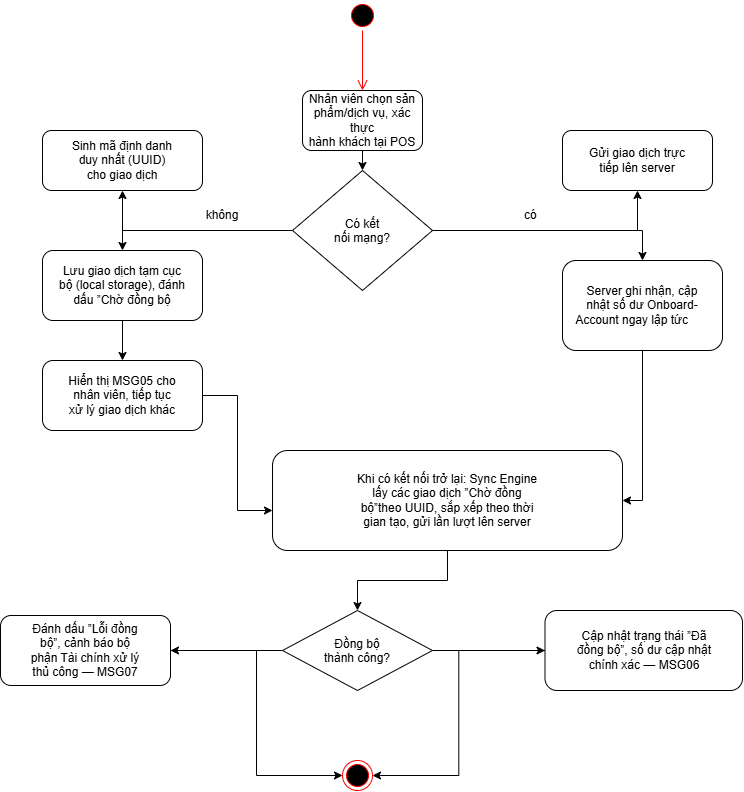
\includegraphics[
        width=0.75\textwidth,
        height=0.72\textheight,
        keepaspectratio
    ]{chapters/ch3/sơ đồ sử lý luồng ngoại tuyến.drawio.png}
\caption{Sơ đồ luồng xử lý giao dịch ngoại tuyến (Offline Transaction Flow)}
\label{fig:offline-transaction-flow}
\end{figure}


\subsubsection{Hủy/hoàn tiền giao dịch}
\textbf{Actor:} Nhân viên bán hàng \& dịch vụ trên tàu (nếu được cấp
quyền)

\textbf{Function description:}
\begin{itemize}
    \item Purpose: Hủy hoặc hoàn tiền một giao dịch đã ghi nhận.
    \item Data processing: Cập nhật trạng thái Transaction thành "Đã
    hủy/Đã hoàn tiền", điều chỉnh lại số dư OnboardAccount.
\end{itemize}

\textbf{Function Details:}
\begin{itemize}
    \item Business Rules: Chỉ nhân viên có quyền "Refund" mới thực hiện
    được; mọi thao tác hủy/hoàn tiền phải ghi log người thực hiện.
\end{itemize}



\subsection{Quản lý Tài khoản trên tàu \& Đối soát (Onboard Account \& Reconciliation)}

\subsubsection{Quản lý tài khoản trên tàu}

\noindent\textbf{Actor:} Tài chính \& Lễ tân

\noindent\textbf{Function description:}
\begin{itemize}
    \item Purpose: Theo dõi số dư và lịch sử giao dịch của từng hành khách/phòng/mã đặt chỗ.
    \item Data processing: Truy vấn OnboardAccount kèm danh sách Transaction liên kết.
\end{itemize}

\noindent\textbf{Function Details:}
\begin{itemize}
    \item Business Rules: Có thể thiết lập hạn mức chi tiêu tối đa cho mỗi tài khoản (credit limit).
\end{itemize}

\begin{figure}[h]
    \centering
    \fbox{%
    \begin{minipage}{0.7\textwidth}
        \centering
        \vspace{2cm}
        \textbf{Mockup màn hình Quản lý tài khoản trên tàu}\\[4pt]
        \footnotesize (placeholder: mockup-onboard-account.png)
        \vspace{2cm}
    \end{minipage}}
    \caption{Mockup màn hình quản lý tài khoản trên tàu}
    \label{fig:mockup-onboard-account}
\end{figure}

\subsubsection{Đối soát giao dịch POS}

\noindent\textbf{Actor:} Tài chính \& Lễ tân

\noindent\textbf{Function trigger:} Chọn "Đối soát" cho một khoảng thời gian/thiết bị POS

\noindent\textbf{Function description:}
\begin{itemize}
    \item Purpose: Kiểm tra khớp giữa giao dịch đã đồng bộ và giao dịch thực tế tại POS, xử lý các giao dịch lỗi đồng bộ.
    \item Data processing: So khớp danh sách Transaction theo POSDeviceId và khoảng thời gian.
\end{itemize}

\noindent\textbf{Function Details:}
\begin{itemize}
    \item Business Rules: Giao dịch lệch số tiền hoặc trùng lặp phải được đánh dấu "Cần xử lý" và không tính vào hóa đơn cuối chuyến cho tới khi được giải quyết.
    \item Normal Case: Toàn bộ giao dịch khớp $\rightarrow$ xác nhận hoàn tất đối soát.
    \item Abnormal Case: Phát hiện sai lệch $\rightarrow$ tạo phiếu tranh chấp (dispute) để xử lý.
\end{itemize}

\subsubsection{Xác nhận thanh toán \& Xuất hóa đơn cuối chuyến}

\noindent\textbf{Actor:} Tài chính \& Lễ tân

\noindent\textbf{Function description:}
\begin{itemize}
    \item Purpose: Chốt số dư cuối cùng và xuất hóa đơn tổng hợp cho hành khách khi kết thúc chuyến đi.
    \item Data processing: Tổng hợp toàn bộ Transaction đã đối soát của một OnboardAccount, tạo bản ghi Invoice.
\end{itemize}

\noindent\textbf{Function Details:}
\begin{itemize}
    \item Validation: Tài khoản phải đã hoàn tất đối soát (không còn giao dịch "Cần xử lý") trước khi xuất hóa đơn.
    \item Business Rules: Hóa đơn cuối chuyến là bất biến (immutable) sau khi xuất, mọi điều chỉnh sau đó phải tạo hóa đơn điều chỉnh riêng.
    \item Normal Case: Xuất hóa đơn thành công, gửi bản sao tới email/app hành khách.
    \item Abnormal Case: Còn giao dịch tranh chấp chưa xử lý $\rightarrow$ hệ thống chặn xuất hóa đơn, hiển thị danh sách cần xử lý.
\end{itemize}

\begin{figure}[h]
    \centering
    \fbox{%
    \begin{minipage}{0.7\textwidth}
        \centering
        \vspace{2cm}
        \textbf{Mockup màn hình Hóa đơn cuối chuyến}\\[4pt]
        \footnotesize (placeholder: mockup-final-invoice.png)
        \vspace{2cm}
    \end{minipage}}
    \caption{Mockup màn hình hóa đơn cuối chuyến}
    \label{fig:mockup-final-invoice}
\end{figure}

% ------------------------------------------------------------

\subsection{Thông báo (Notification Management)}

\subsubsection{Gửi thông báo tự động}

\noindent\textbf{Actor:} Hệ thống (tự động), Điều phối lịch trình

\noindent\textbf{Function description:}
\begin{itemize}
    \item Purpose: Gửi thông báo về thay đổi lịch trình, giờ tập trung, giờ quay lại tàu tới hành khách liên quan.
    \item Data processing: Tạo bản ghi Notification, gửi qua push notification (Mobile App) và/hoặc email.
\end{itemize}

\noindent\textbf{Function Details:}
\begin{itemize}
    \item Business Rules: Thông báo liên quan tới an toàn (giờ quay lại tàu) phải được đánh dấu mức độ ưu tiên cao và gửi lặp lại nếu chưa được xác nhận đã đọc.
\end{itemize}

% ------------------------------------------------------------

\subsection{Dashboard Vận hành (Operations Dashboard)}

\subsubsection{Xem dashboard vận hành}

\noindent\textbf{Actor:} Quản lý vận hành

\noindent\textbf{Function description:}
\begin{itemize}
    \item Purpose: Cung cấp cái nhìn tổng quan về hoạt động, dịch vụ, doanh thu, sức chứa theo thời gian thực.
    \item Data processing: Tổng hợp dữ liệu từ Activity, ShoreExcursion, Transaction, Registration.
\end{itemize}

\noindent\textbf{Function Details:}
\begin{itemize}
    \item Business Rules: Dữ liệu dashboard có độ trễ tối đa bằng thời gian đồng bộ ngoại tuyến (không đảm bảo 100\% real-time trong điều kiện mạng kém).
\end{itemize}

\begin{figure}[h]
    \centering
    \fbox{%
    \begin{minipage}{0.7\textwidth}
        \centering
        \vspace{2cm}
        \textbf{Mockup Dashboard vận hành}\\[4pt]
        \footnotesize (placeholder: mockup-operations-dashboard.png)
        \vspace{2cm}
    \end{minipage}}
    \caption{Mockup Dashboard vận hành}
    \label{fig:mockup-dashboard}
\end{figure}

\subsubsection{Giám sát check-in / rủi ro quay lại tàu muộn}

\noindent\textbf{Actor:} Quản lý vận hành

\noindent\textbf{Function description:}
\begin{itemize}
    \item Purpose: Theo dõi danh sách hành khách chưa check-in quay lại tàu sau giờ hẹn.
    \item Data processing: So sánh danh sách hành khách đã rời tàu (ghi nhận qua check-out tham quan bờ) với danh sách đã check-in quay lại.
\end{itemize}

\noindent\textbf{Function Details:}
\begin{itemize}
    \item Business Rules: Cảnh báo tự động (highlight đỏ) khi hành khách trễ quá X phút so với giờ tàu rời bến đã thiết lập.
\end{itemize}

% ------------------------------------------------------------

\subsection{Quản trị Hệ thống (System Administration)}

\subsubsection{Quản lý người dùng}

\noindent\textbf{Actor:} Quản trị viên hệ thống

\noindent\textbf{Function description:}
\begin{itemize}
    \item Purpose: CRUD tài khoản, phân quyền theo vai trò.
    \item Data processing: Tạo/sửa/xóa bản ghi User, gán Role.
\end{itemize}

\noindent\textbf{Function Details:}
\begin{itemize}
    \item Business Rules: Không được xóa cứng (hard delete) tài khoản đã có lịch sử giao dịch, chỉ vô hiệu hóa (soft delete).
\end{itemize}

\subsubsection{Cấu hình chính sách hệ thống}

\noindent\textbf{Actor:} Quản trị viên hệ thống

\noindent\textbf{Function description:}
\begin{itemize}
    \item Purpose: Thiết lập chính sách đăng ký, hủy, hoàn tiền áp dụng chung cho toàn hệ thống.
\end{itemize}

\noindent\textbf{Function Details:}
\begin{itemize}
    \item Business Rules: Thay đổi chính sách chỉ áp dụng cho các giao dịch phát sinh sau thời điểm cập nhật, không hồi tố.
\end{itemize}

\subsubsection{Quản lý thiết bị QR/RFID/NFC/BLE}

\noindent\textbf{Actor:} Quản trị viên hệ thống

\noindent\textbf{Function description:}
\begin{itemize}
    \item Purpose: Quản lý danh sách thiết bị xác thực, gán/thu hồi thiết bị cho hành khách hoặc trạm POS.
\end{itemize}

\noindent\textbf{Function Details:}
\begin{itemize}
    \item Business Rules: Thiết bị bị báo mất phải được vô hiệu hóa ngay để tránh sử dụng gian lận tài khoản trên tàu.
\end{itemize}

% ------------------------------------------------------------

\subsection{Module Định vị Hành khách qua BLE (tùy chọn / nâng cao)}

\subsubsection{Gán thiết bị BLE cho hành khách}

\noindent\textbf{Actor:} Quản trị viên hệ thống

\noindent\textbf{Function description:}
\begin{itemize}
    \item Purpose: Gán thiết bị đeo BLE cho hành khách sử dụng (tùy chọn, không bắt buộc).
\end{itemize}

\noindent\textbf{Function Details:}
\begin{itemize}
    \item Business Rules: Hành khách phải đồng ý (opt-in) sử dụng tính năng định vị trước khi thiết bị được kích hoạt.
\end{itemize}

\subsubsection{Ghi nhận vị trí hành khách}

\noindent\textbf{Actor:} Hệ thống (tự động)

\noindent\textbf{Function description:}
\begin{itemize}
    \item Purpose: Ước tính vị trí hành khách ở mức khu vực (zone) trên tàu, hỗ trợ tìm kiếm và an toàn khẩn cấp.
    \item Data processing: Nhận tín hiệu từ BLE receiver, ghi log LocationLog theo khu vực gần nhất.
\end{itemize}

\noindent\textbf{Function Details:}
\begin{itemize}
    \item Business Rules: Dữ liệu vị trí chỉ chính xác ở mức khu vực, không phải tọa độ chính xác tuyệt đối.
\end{itemize}


